\documentclass[11pt,a4paper]{article}

\usepackage[spanish,es-nodecimaldot]{babel}
\usepackage[T1]{fontenc}
\usepackage[utf8]{inputenc}
\usepackage{lmodern}
\usepackage{geometry}
\usepackage{graphicx}
\usepackage{float}
\usepackage{hyperref}
\usepackage{enumitem}

\geometry{margin=2.5cm}
\hypersetup{colorlinks=true,linkcolor=black,urlcolor=blue}
\graphicspath{{img/}}

\title{Firma digital}
\author{Javier Siñuka}
\date{11 de septiembre de 2026}

\begin{document}

\maketitle

\section{Objetivo}

El objetivo de esta tarea fue configurar el uso de firma digital en un cliente
de correo y emplear cifrado para intercambiar mensajes con un compañero. La
práctica permite comprobar, en un caso de uso cotidiano, las propiedades que
ofrece la criptografía asimétrica: autenticidad, integridad y confidencialidad.

En particular, se realizaron las siguientes actividades:

\begin{itemize}[noitemsep]
    \item configurar el cliente de correo para utilizar OpenPGP y una clave
    personal;
    \item intercambiar un correo firmado para disponer de la clave pública del
    compañero;
    \item enviar y recibir un correo cifrado, verificando el resultado tanto
    en la interfaz web del proveedor como en el cliente de correo.
\end{itemize}

\section{Conceptos utilizados}

La firma digital se genera con la \emph{clave privada} del remitente. El
receptor la valida con la \emph{clave pública} correspondiente; de este modo
puede comprobar quién firmó el mensaje y detectar modificaciones posteriores.
La clave privada no se comparte.

El cifrado, en cambio, busca preservar el secreto del contenido. Para enviar
un mensaje al compañero, el remitente cifra usando la clave pública de éste;
solamente el destinatario, que posee la clave privada asociada, puede
descifrarlo. OpenPGP permite combinar ambos mecanismos en un mismo mensaje:
se firma para aportar autenticidad e integridad y se cifra para aportar
confidencialidad.

\section{Procedimiento realizado}

\subsection{Configuración e intercambio de claves}

Se habilitó OpenPGP en el cliente de correo y se configuró la identidad del
usuario con su par de claves. Para poder enviar un mensaje cifrado, fue
necesario contar previamente con la clave pública del destinatario. Esta clave
se obtuvo mediante el intercambio de un correo firmado con el compañero
Agustín Tosolini. Una vez asociada la clave pública con su dirección de correo,
el cliente pudo cifrar los mensajes dirigidos a dicho destinatario.

Esta separación es importante: el proveedor de correo transporta el mensaje,
pero las operaciones criptográficas se realizan con las claves OpenPGP de los
usuarios. Por ello, enviar un correo firmado permite al receptor verificar la
identidad criptográfica del emisor, mientras que el correo cifrado requiere la
clave pública del receptor antes de su envío.

\subsection{Envío y recepción del correo cifrado}

Se envió un mensaje de prueba desde la cuenta de Javier S. y se recibió la
respuesta del compañero. En la interfaz web del proveedor se observa el correo
recibido y los adjuntos generados para el intercambio: un archivo de clave y
el archivo \texttt{encrypted.asc}. La extensión \texttt{.asc} corresponde a
una representación ASCII habitual de los datos protegidos con OpenPGP.

\begin{figure}[H]
    \centering
    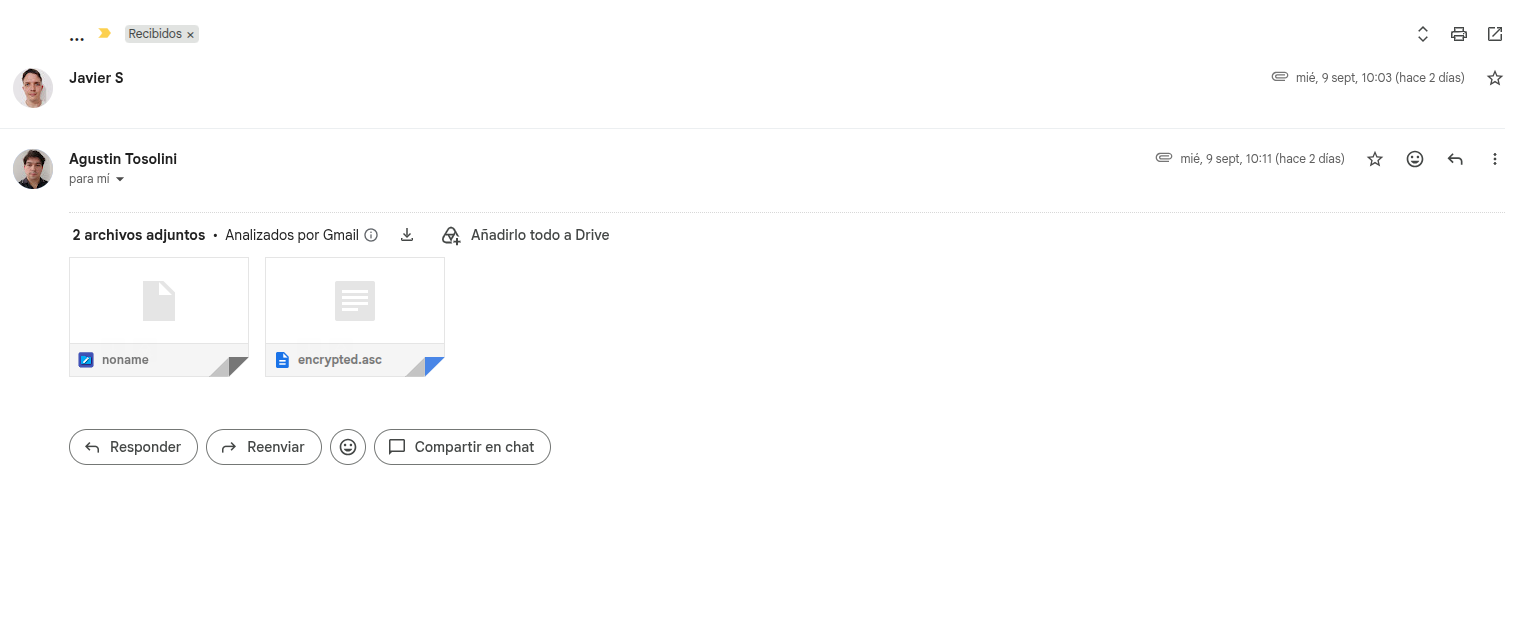
\includegraphics[width=\textwidth]{Screenshot from 2026-09-11 09-53-51.png}
    \caption{Correo mostrado en la interfaz web de Gmail. Se visualizan los
    adjuntos del intercambio, incluido el archivo cifrado \texttt{encrypted.asc}.}
    \label{fig:gmail}
\end{figure}

Posteriormente, el mismo intercambio se abrió en el cliente de correo. La
Figura~\ref{fig:cliente} muestra el contenido legible del mensaje y los
indicadores de OpenPGP en la cabecera. Esto evidencia que el cliente reconoció
el mensaje protegido y pudo procesarlo con el material criptográfico disponible
para la cuenta receptora.

\begin{figure}[H]
    \centering
    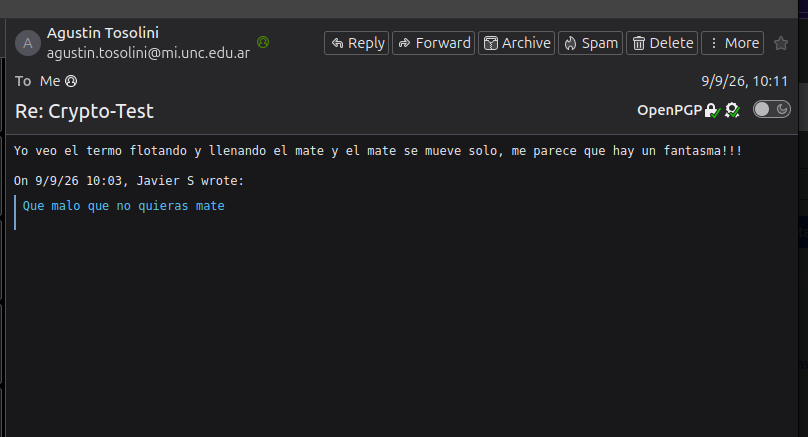
\includegraphics[width=0.78\textwidth]{Screenshot from 2026-09-11 09-52-32.png}
    \caption{Mensaje abierto en el cliente de correo. La cabecera presenta los
    indicadores de OpenPGP y el contenido puede leerse luego del procesamiento
    criptográfico.}
    \label{fig:cliente}
\end{figure}

\clearpage
\section{Firma digital en la provincia de Córdoba}

Sí, es posible obtener una firma digital con validez legal en la provincia de
Córdoba. El trámite debe realizarse ante una Autoridad de Registro habilitada
por la Autoridad Certificante de la República Argentina. En términos generales,
el solicitante debe iniciar la solicitud del certificado, acreditar su identidad
de manera presencial o mediante el mecanismo de validación que establezca la
autoridad correspondiente y aceptar las condiciones de emisión. El certificado
resultante vincula la identidad verificada con una clave pública.

Una alternativa práctica es la Firma Digital Remota sin token: se solicita un
turno ante la Autoridad de Registro más cercana, se presenta el DNI, CUIL/CUIT,
un correo electrónico y un teléfono con aplicación para generar códigos de un
solo uso (OTP). El sitio oficial nacional indica que el trámite no tiene costo
para el solicitante. En Córdoba existen certificadores y puntos de atención
habilitados; su disponibilidad debe verificarse antes de pedir turno en el
listado oficial de Autoridades de Registro~\cite{pfdr,certificadores}.

Debe distinguirse esta firma digital basada en certificado de la configuración
OpenPGP utilizada en esta práctica. Ambas emplean criptografía de clave pública,
pero la primera se integra a la infraestructura de certificación estatal para
otorgar efectos jurídicos, mientras que OpenPGP se utilizó aquí para proteger y
autenticar correos entre usuarios.

\section{Conclusiones}

La práctica permitió configurar OpenPGP en el cliente de correo, intercambiar
la información necesaria para identificar la clave pública del compañero y
verificar el envío de un correo cifrado. Las capturas confirman las dos vistas
solicitadas: en la interfaz web se aprecia el mensaje y su archivo cifrado; en
el cliente de correo se aprecia el mensaje procesado junto con los indicadores
OpenPGP. De este modo, el uso conjunto de firma y cifrado aporta autenticidad,
integridad y confidencialidad al intercambio de correo electrónico.

\begin{thebibliography}{9}
\bibitem{pfdr}
República Argentina, \emph{Solicitar Firma Digital Remota sin Token}.
\url{https://www.argentina.gob.ar/node/115431}.

\bibitem{certificadores}
República Argentina, \emph{Certificadores Licenciados}.
\url{https://www.argentina.gob.ar/jefatura/innovacion-ciencia-y-tecnologia/innovacion/firma-digital/certificadores-licenciados}.
\end{thebibliography}

\end{document}
